% https://academy.ifcopenshell.org/posts/using-ifcopenshell-and-pythonocc-to-generate-cross-sections-directly-from-an-ifc-file/
% https://blenderbim.org/docs-python/ifcopenshell-python/geometry_processing.html
%https://academy.ifcopenshell.org/posts/using-ifcopenshell-and-pythonocc-to-construct-new-geometry/

\chapter{Grundlagen}\label{basics}
Zunächst wird für diese Arbeit ein geeignetes Speicherformat für 3D Modelle von Gebäuden benötigt.
Um den Bau von Gebäuden zu automatisieren, ist es notwendig die Domäne \textit{Gebäude} möglichst vollständig digital abbilden zu können. 
Hilfreich ist dabei, wichtige Daten über bestimmte Bestandteile des Gebäudes direkt in das Modell zu integrieren, auf Basis derer etwa Kostenberechnungen durchgeführt oder Materialmengen herausgefunden werden können.
Da diese Informationen oft von Experten verschiedener Fachbereiche (etwa aus den Bereichen der Architektur, des Bauwesens oder der Statik) stammen, muss das Format sehr flexibel und im besten Fall auch zeitgleich bearbeitbar sein.
Dafür werden seit dem Jahr 2000 die \textit{Industry Foundation Classes} (IFC) von buildingsmart entwickelt, deren Anwendung im internationalen Bauwesen mittlerweile weit verbreitet ist~\cite{Industry61:online}.


\section{Industry Foundation Classes}\label{basics:ifc}
In der Spezifikation des Standards selbst, wird dieser wie folgt beschrieben:
\glqq{}Die Industry Foundation Classes (IFC) sind ein offener internationaler Standard für Daten des Building Information Model (BIM), welche zwischen Softwareanwendungen ausgetauscht, gemeinsam genutzt und von den verschiedenen Akteuren der Bauindustrie und des Gebäudemanagements verwendet werden. 
Der Standard enthält Definitionen für Daten, die für die Lebenszyklen von Gebäude- und Infrastrukturarbeiten erforderlich sind. 
Die bis jetzt in die IFC aufgenommenen Infrastrukturtypen umfassen Brücken, Straßen, Eisenbahnen, Wasserstraßen und Hafenanlagen\grqq{} (aus dem Englischen)~\cite{IFCScope:online}. 
Eine frühere Version des IFC Standards ist unter der Bezeichnung ISO 16739 registriert (siehe~\cite{ISOISO1694:online}).
Da die IFC aber nach wie vor kontinuierlich weiterentwickelt werden, wird in dieser Arbeit die derzeit neueste Version verwendet.
Diese ist die IFC Spezifikation 4.3.1.0~\cite{IFC4310Spezification:online}.
Das verbreitetste Austauschformat für IFC ist das Step Physical File Format, welches im ISO 10303 Teil 21 registriert ist~\cite{ISO_Step:online}.
Zudem gibt es speicherreduzierte Formate wie ifcZip oder für Menschen lesbarere Formate wie ifcXML~\cite{Industry93:online}\cite{IFCForma28:online}\cite{BIM_handbook_AEC_XML_SCHEMAS}.

\subsection{IFC 4.3.1.0 Aufbau}
Im Grunde definieren die \textit{Industry Foundation Classes} eine Vielzahl an Klassen, die in einer komplexen Hierarchie angeordnet den Grundstock des Datenmodells bilden.
Diese sind anfangs abstrakte Konzepte, die sich mit zunehmender Tiefe in der Hierarche konkretisieren.
\begin{figure}[ht]
    \centering
    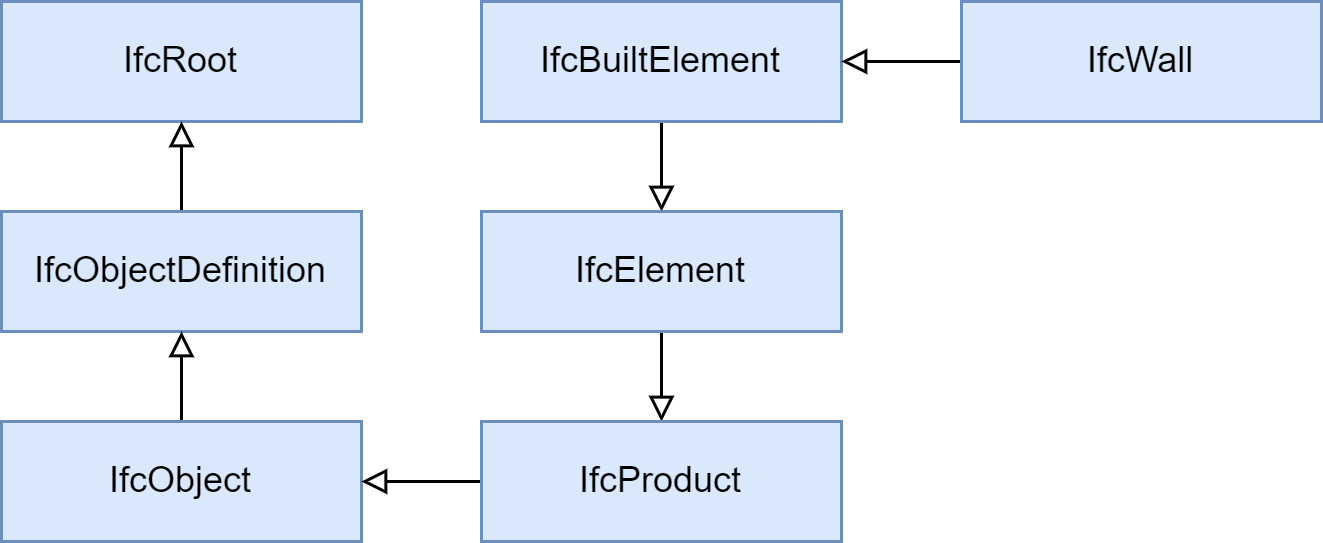
\includegraphics[width=0.6\columnwidth]{fig/Hierarchie_IfcWall_300.drawio.png}
    \caption{Klassenhierarchie am Beispiel der Klasse \textit{IfcWall}}
    \label{fig:IfcWall_Hierarchie}
\end{figure}
Da sich diese Arbeit zum größten Teil mit aus Wänden bestehenden Gebäuden befasst, wird nachfolgend die Klasse \textit{IfcWall} wiederholt als Beispiel herangezogen.
Der für diese Klasse relevante Ausschnitt aus der Klassenhierarchie ist in Abbildung~\ref{fig:IfcWall_Hierarchie} dargestellt.
Objekte werden von dem Standard in Relation zueinander gestellt, um komplexere Zusammenhänge darzustellen.
In Abbildung~\ref{fig:IFC_Relationships} erkennt man den Zusammenhang zwischen einem Objekt des Types \textit{IfcWall}, des Stockerwerks, welches diese Wand referenziert und wiederum selbst Teil eines \textit{IfcBuildings} ist, bis hin zur obersten Komponente eines Ifc Projektes, dem gleichnamigen \textit{IfcProject}.

\begin{figure}[h]
    \centering
    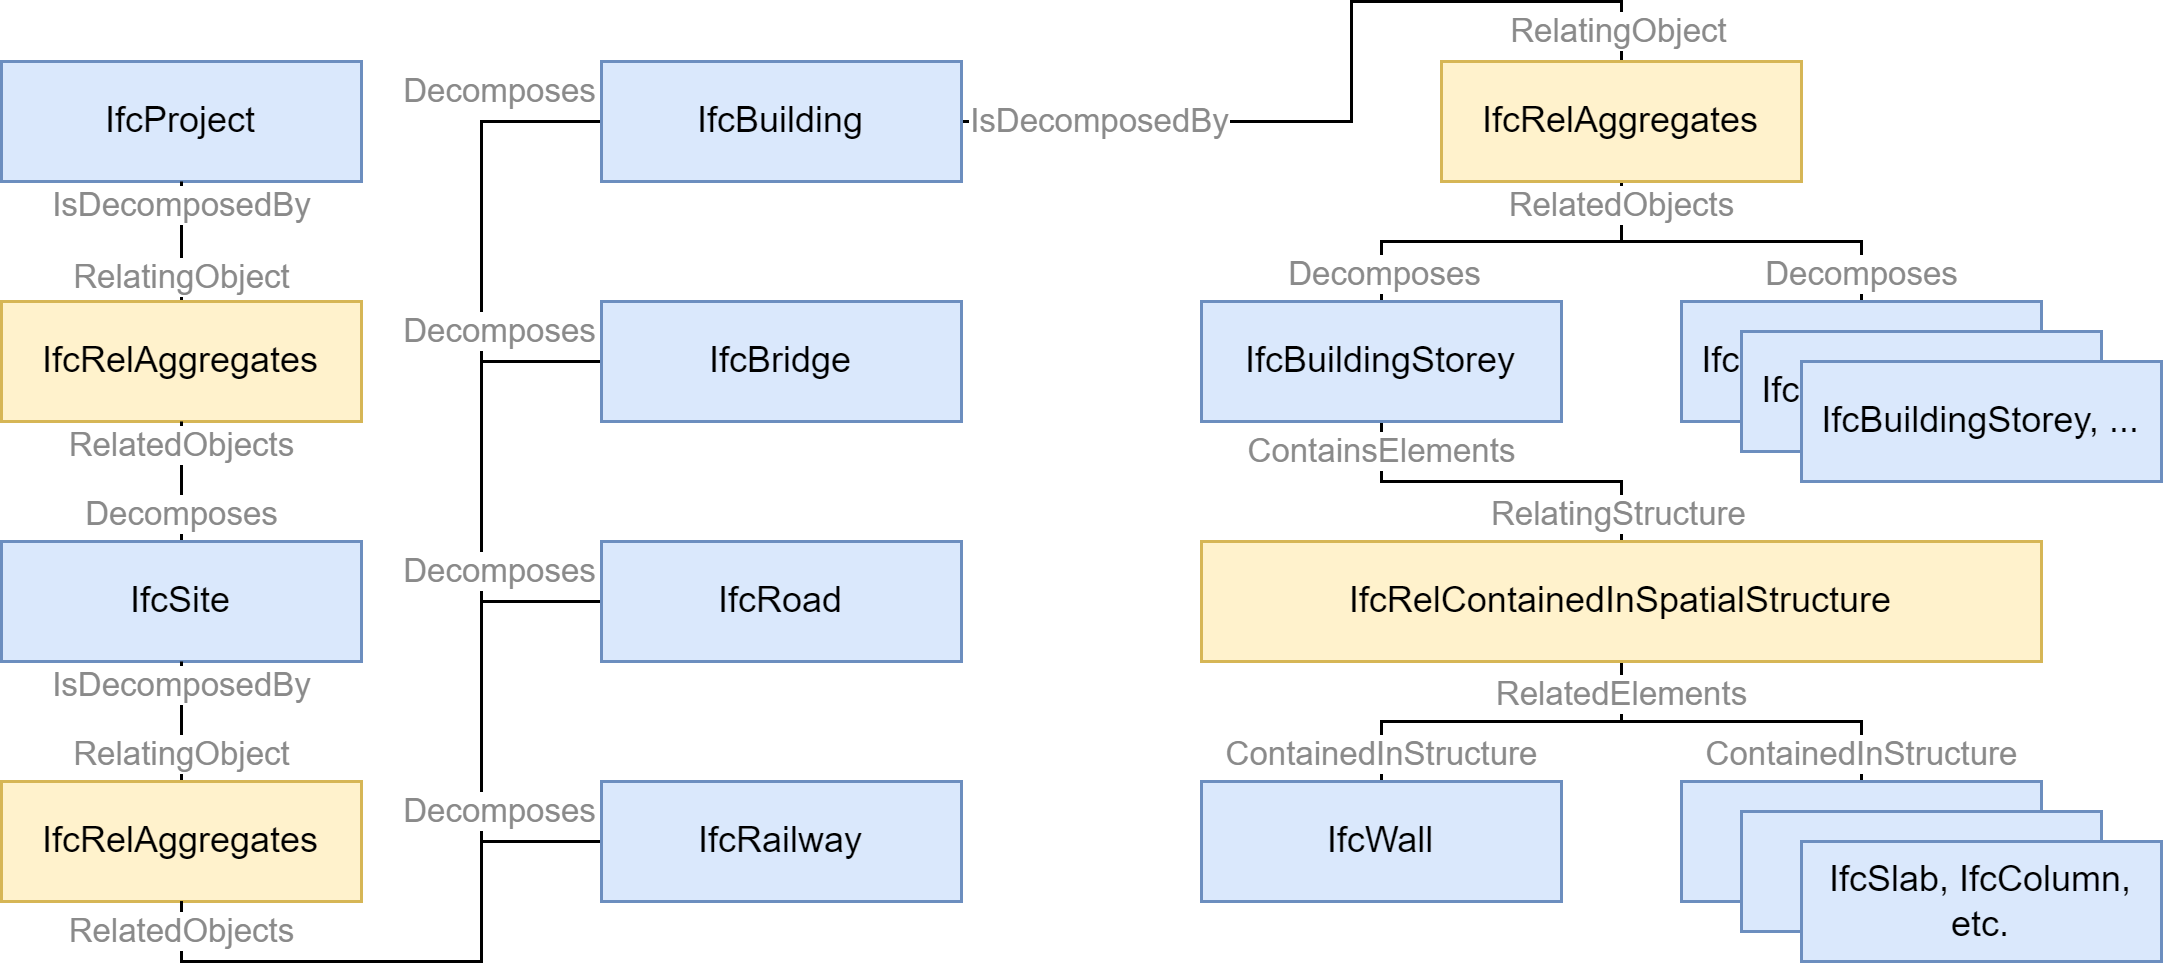
\includegraphics[width=0.9\columnwidth]{fig/IFC_Relationships_300.drawio.png}
    \caption{Relation der IfcWall und einem \textit{IfcProject}}
    \label{fig:IFC_Relationships}
\end{figure}

\subsection{IfcPropertySets und IfcQuantitySets}\label{basics:ifc_properties}
Mit dem Erweitern des Gebäudemodells um möglichst viele Informationen, schafft man einen detailierten digitalen Zwilling, der neben der bloßen Darstellung des Gebäudes als 3D Modell zusätzlich die Untersuchung auf andere Eigenschaften ermöglicht.
Dazu zählen zum Beispiel eine präzisere Kosten- und Zeitschätzung, Sicherheitsaspekte und Emissionen eines Bauvorhabens~\cite{Industry93:online}~\cite{Ding2014}. 
Dies ist mithilfe von \textit{IfcPropertySets} und \textit{IfcQuantitySets} umsetzbar, welche Objekten oder Objekttypen angehängt werden können.
Dabei werden IfcQuantitySets vorwiegend dazu verwendet numerische Werte zu geometrischen oder physikalischen Eigenschaften auszudrücken.
IfcPropertySets dienen hingegen dazu bestimmten Objekten oder Objekttypen mit sämtlichen nicht numerischen Werten zu annotieren.
Beispiele dafür sind etwa Material oder Farbe eines bestimmten Objekts.
Die Verwendung der Bezeichnung \textit{Set} rührt daher, dass diese Informationen in einer Baumstruktur vorliegen und demnach verschachtelt sein können.
Es gibt zu vielen Klassenbeschreibungen des IFC Standards vordefinierte PropertySets.
Das hilft dabei wichtige Informationen zu bestimmten Objekttypen einheitlich angeben zu können.
Im Falle des \textit{IfcWallType} existiert beispielsweise das PropertySet mit dem Namen \textit{Pset\_WallCommon}~\cite{IFC4310PSetWallCommon:online}.
Darin können die Ersteller von neuen WallTypes unter anderem Informationen über Brennbarkeit, thermisches Verhalten oder Akustik hinterlegen.
Bei Erstellen einer IfcWall-Instanz aus einem bestimmten WallType werden die damit verbundenen Property- und QuantitySets automatisch daran angehängt, sodass jedes Objekt relevante Informationen über sich selbst bereithält.

\subsection{Positionierung von IFCProducts}
%https://ifc43-docs.standards.buildingsmart.org/IFC/RELEASE/IFC4x3/HTML/concepts/Product_Shape/Product_Placement/Product_Local_Placement/content.html
%https://community.osarch.org/discussion/654/how-to-extract-location-data-from-ifc mal schauen ob man das easy machen kann mit openshell
TODO: Positionierung ist anscheinend bisschen verschachtelt
Blablabla so können aus einem IFC Projekt alle relevanten Klassen mit den für diese Arbeit erforderlichen Eigenschaften extrahiert werden.
This is a test

\subsection{IfcOpeningElement}
\label{basics:IfcOpeningElement}
Neben Wänden stellen Fenster und Türen wichtige Elemente eines Gebäudes dar.
Diese sind ebenfalls Teil der Klassen des IFC Standards.
Objekte des Typs \textit{IfcOpeningElement} dienen dazu die notwendigen Lücken in einer Wand zu definieren in die später eine Tür oder ein Fenster eingebaut werden soll.
In der Dokumentation wird dies wie folgt formuliert (aus dem Englischen): \glqq{}[Das IfcOpeningElement] stellt eine Lücke in jedem Element dar, das eine physische Manifestation hat\grqq{}~\cite{IFC4310OpeningElement:online}.
Es gibt zwei Arten an IfcOpeningElement, je nachdem ob die Öffnung durch die gesamte Breite eines Objektes reicht oder nicht. 
Folglich entsteht dadurch eine Unterscheidung zwischen Nischen und tatsächlichen Öffnungen, wobei nur letztere im Zusammenhang mit Fenstern oder Türen Sinn ergibt.
TODO: Diagramm zwischen IFCWall und IfcOpeningElement.

\section{IFC for Blender}\label{basics:blender}
\subsection{Blender}
Blender ist eines der beliebtesten Open Source Programme zur Modellierung von 3D Modellen und Animationen~\cite{blendero56:online}.
Eine umfangreiche Python API erlaubt es Blender durch sogenannte Addons an die eigenen Bedürfnisse anzupassen~\cite{PythonWebsite:online}~\cite{BlenderPythonAPI:online}.
Aufgrund dessen existiert auch eine Vielzahl an freien Erweiterungen \textendash{} unter anderem auch eine Integration von IFC Projekten.

\subsection{blenderbim}
Neben kommerziellen Produkten wie etwa revit von autodesk zur Modellierung von IFC Modellen, gibt es auch für Blender ein freies Plugin, um IFC Modelle zu erstellen~\cite{RevitSof26:online}~\cite{BlenderB43:online}.
Dieses Plugin ermöglicht es neben dem bloßen Designen des Gebäudes in kurzer Zeit z.B. detailierte Zeichnungen verschiedener Perspektiven herauszuarbeiten, die z.B. von Bauingeneuren verwendet werden können, um einzelne Stockwerke oder Verkabelungen zu planen.
Blenderbim selbst kapselt unter anderem die Open Source Python Bibliothek \textit{IfcOpenShell}, sodass diese in der Blender Laufzeitumgebung zur Verfügung steht \cite{IFCOpenShell:online}.

\subsection{IfcOpenShell}\label{basics:ifcopenshell}
\begin{lstlisting}[label={basics:ifcopenshell_sample_code}, language=Python, caption=Beispielprogramm zur Extraktion bestimmter Daten einer IFC Datei und Generierung eines Meshes aus deren geometrischen Representationen.]
import ifcopenshell
from ifcopenshell import geom
from stl import mesh, Mode
import numpy as np

settings = ifcopenshell.geom.settings()
settings.set(settings.USE_WORLD_COORDS, True)

ifc_file = ifcopenshell.open("model.ifc")
products = ifc_file.by_type("IfcProduct")
meshes = []

for product in products:
    if product.Representation and product.is_a("IfcWall"):
        shape = ifcopenshell.geom.create_shape(settings, product)
        vertices = np.array(shape.geometry.verts).reshape((-1, 3))
        edges = np.array(shape.geometry.edges)
        faces = np.array(shape.geometry.faces).reshape((-1, 3))

        m = mesh.Mesh(np.zeros(faces.shape[0], dtype=mesh.Mesh.dtype))
        for i, f in enumerate(faces):
            for j in range(3):
                m.vectors[i][j] = vertices[f[j], :]
        meshes.append(m)

# Create the combined mesh
combined = mesh.Mesh(np.concatenate([m.data for m in meshes]))
combined.save('model.stl', mode=Mode.ASCII)
\end{lstlisting}

IfcOpenShell ist eine frei verfügbare Bibliothek, die es erleichtert mit Daten im IFC Format zu arbeiten.
Sie bietet unter anderem eine Python API an und ist wie bereits erwähnt ein Teil des Blender Addons blenderbim.
Natürlich ist es dennoch möglich diese Bibliothek auch ohne Blender zu verwenden.
In Listing~\ref{basics:ifcopenshell_sample_code} ist ein kurzes Beispiel eines Programmes gegeben, das in einer IFC Datei alle Objekte des Typs IfcWall ausfindig macht und dessen geometrische Representation in ein herkömmliches Mesh konvertiert.
Damit existiert ein intuitiver Zugang zu den Daten von IFC Dateien.

\section{Building Information Modeling}\label{basics:bim}
Ein weiterer Punkt, der für die Verwendung von IFC spricht ist das sogenannte \textit{Building Information Modeling} (BIM)~\cite{Building41:online}.
Ein Definitionsvorschlag lautet wie folgt: \glqq{}BIM ist definiert als der Einsatz von Informations- und Kommunikationstechnologien zur Verschlankung der Prozesse im Lebenszyklus von Gebäuden, um eine sicherere und produktivere Umgebung für die Bewohner zu schaffen, die Umwelt so wenig wie möglich zu belasten und die Effizienz der Betriebsabläufe für die Eigentümer während des gesamten Lebenszyklus des Gebäudes zu erhöhen\grqq{} (Übersetzt aus dem Englischen)~\cite{Microsof51:online}.
Zum Lebenszyklus eines Gebäudes gehören etwa anfangs das Planen und Designen, später das Bauen, das Verwenden und Instandhalten und nach eventuellen Renovierungen das Abreißen.
BIM kommt in all diesen Phasen zum Tragen und erleichtert diese Prozesse durch Anbieten einer einheitlichen Schnittstelle für alle am Infrastrukturbau und -management beteiligten Personen.
Zusätzlich ermöglicht BIM eine exakte Dokumentation des Geschehens in sämtlichen Phasen des Bauwerks, was unter anderem zu einer genaueren Zeit- und Kostenplanung führt~\cite{Ding2014}.
Auch Verantwortlichkeiten sind Teil von BIM, was zu einer erhöhten Produktivität beiträgt.
Um nun das Zusammenarbeiten der unterschiedlichen Fachbereiche zu erleichtern, gibt es sogennante BIM-Server auf welchen mehrere Arbeitende synchron an einem Projekt arbeiten können, während sie jeweils die für ihren Aufgabenbereich passende Ansicht vor sich haben.
BIM-Server unterstützen zusätzlich eine Versionierung des Fortschritts an einem Projekt.

In einem Gespräch mit einem Ingeneur aus dem Bereich \glqq{}Energysystemtechnik\grqq{} kam zur Sprache, dass viele Bereiche von BIM noch nicht ganz Einzug in Deutschland gefunden haben.
Eben jene \glqq{}Kollaboration über einen BIM-Server mit Änderungsmanagement etc. [sei] (noch) nicht üblich, da noch nicht alle Beteiligten dazu in der Lage sind. Vor allem Bauherren, Architekten und Baufirmen können es nicht\grqq{}.
Weiter sei \glqq{}auch unklar, wer für falsche Angaben haftet und wer die Konsistenz aller Daten gewährleistet\grqq{}.
Auf der anderen Seite sei \glqq{}das im BIM festegelegte Datenformat IFC das Maß der Dinge und auch bei uns so in Verwendung\grqq{}.
Auch das Einpflegen \glqq{}ergänzende[r] Bauteilinformationen (z.B. zu Gewicht, Dämmwert, Recyclebarkeit, CO2 Fußabdruck, etc.)\grqq{} finden Einsatz und sind Teil seines Alltags.
Für ihn wichtig ist ebenfalls der Betrieb des Gebäudes.
Hier unterstützt BIM, indem sämtliche Teile der Installationen in einem Gebäude, wie z.B Fensterdichtungen, Kabel, Rohre, Sicherungen oder eine Umwälzpumpe individuelle Teilenummern zugewiesen bekommen, hinter welchen alle Daten wie etwa Hersteller, Bestellnummern, Lebensdauer, Wartungshistorie oder Entsorgungsnachweise vermerkt sind.
Dies wurde allerdings \glqq{}angesichts der Realität der Handwerker und Gebäudenutzer für völlig unrealisitsch und auch etwas over-engineered\grqq{} eingestuft.
Trotzdem sei \glqq{}BIM [\ldots] das große Ding in der Bauwelt und der einzige echte Standard\grqq{}.

\section{opensourcebim}
Während es vorwiegend kommerzielle Produkte gibt, die Unternehmen das Arbeiten mit BIM ermöglichen, exisitiert auch hier eine aktive Open Source Bewegung.
Unter dem Namem \glqq{}The open source BIM collective\grqq{} oder kurz \glqq{}opensourceBIM\grqq{} werden derzeit um die 70 Repositories betrieben.
Darin enthalten sind unter anderem ein BIM-Server inklusive verschiedener Clients für Endanwender auf unterschiedlichen Systemen und Werkzeuge, die es erleichtern den IFC Files zu arbeiten~\cite{Theopens96:online}.
Ein kurzer Test hat gezeigt, dass die in Blender modellierte IFC Files tatsächlich über einen \glqq{}Anzeige-Client\grqq{}, der mit einem lokal gehosteten BIM-Server verbunden ist, angezeigt werden können.
Obwohl die Verwendung des BIM-Servers für diese Arbeit nicht notwendig ist, besteht die Option diesen künftig mit in den Workflow zu integrieren, da damit auch das simultante Arbeiten an einem IFC File möglich ist, was in Blender nur teilweise und mit dem Einsatz von Plugins ermöglicht wird.
Das stellt einen Praxisbezug zum aktuell verwendeten Stand dieser Technologien her, was in der oftmals konzeptionellen Natur der Forschung nicht immer der Fall ist.
Wie auch Blender untertützt BIM-Server das Einbinden von eigenen Plugins, sodass eine Erweiterung um neue Funktionalität möglich ist.
Die Plugins werden in Java geschrieben.
Der Server bietet aber auch eine REST Schnittstelle an, um Clients in anderen Sprachen anzubinden.

\section{Mauerwerksbau}
\label{basics: Mauerwerksbau}
Der Mauerwerksbau ist eine Art des Massivbaus, bei welchem Natur- oder Formsteine aufgeschichtet werden, um Wände beziehungsweise Mauern zu errichten.
Eine derart erbaute Wand besteht demnach aus (Bau)-Steinen und den dazwischen entstehenden Fugen.
Mörtel ist dabei nicht zwangsläufig notwendig.
Man spricht von trocken versetzten Steinen oder einer Trockenmauer, wenn darauf verzichtet wird.
Heutzutage wird fast ausschließlich mit quaderförmigen Formsteinen gebaut.
Zur Beschreibung solcher Formsteine existieren zwei relevante Größen.
Die eine ist das sogenannte \textit{Baunennmaß}, mit dem die tatsächliche Größe des Steins angegeben wird.
Die andere das \textit{Baurichtmaß}, das sich aus Baunennmaß und dem Fugenmaß zusammensetzt.

\subsection{Maßsysteme}
Als Maßsystem bezeichnet man das Vorgeben der Größen von Bausteinen anhand eines konkret definierten (Grund-)Moduls.
Zwei in Deutschland populäre Grundmodule sind zum einem das \textit{ISO-2848-Basismodul} mit Länge 100mm und zum anderen der Achtelmeter, verankert in der \textit{DIN 4172 Maßordnung im Hochbau}~\cite{ISO2848}\cite{DIN417224}.
Letzteres bezeichnet man daher auch als das oktametrische Maßsystem.
Nachfolgend wird auf dieses Maßsystem näher eingegangen.

\subsubsection*{Oktametrisches Maßsystem}
Baurichtmaße sind gemäß dem oktametrischen Maßsystem immer ein Vielfaches von \(12,5 cm\) (das entspricht \(1/8 m\)) und nach der Norm aber mindestens \(6.25cm\).
Dies gilt sowohl für Länge und Breite als auch für die Höhe der Steine.
Das System ist in der \textit{DIN 4172 Maßordnung im Hochbau} geregelt und ist ein fest definiertes Grundmaß für das Bauwesen in Europa~\cite{DIN417224}.
\begin{figure}[ht]
    \centering
    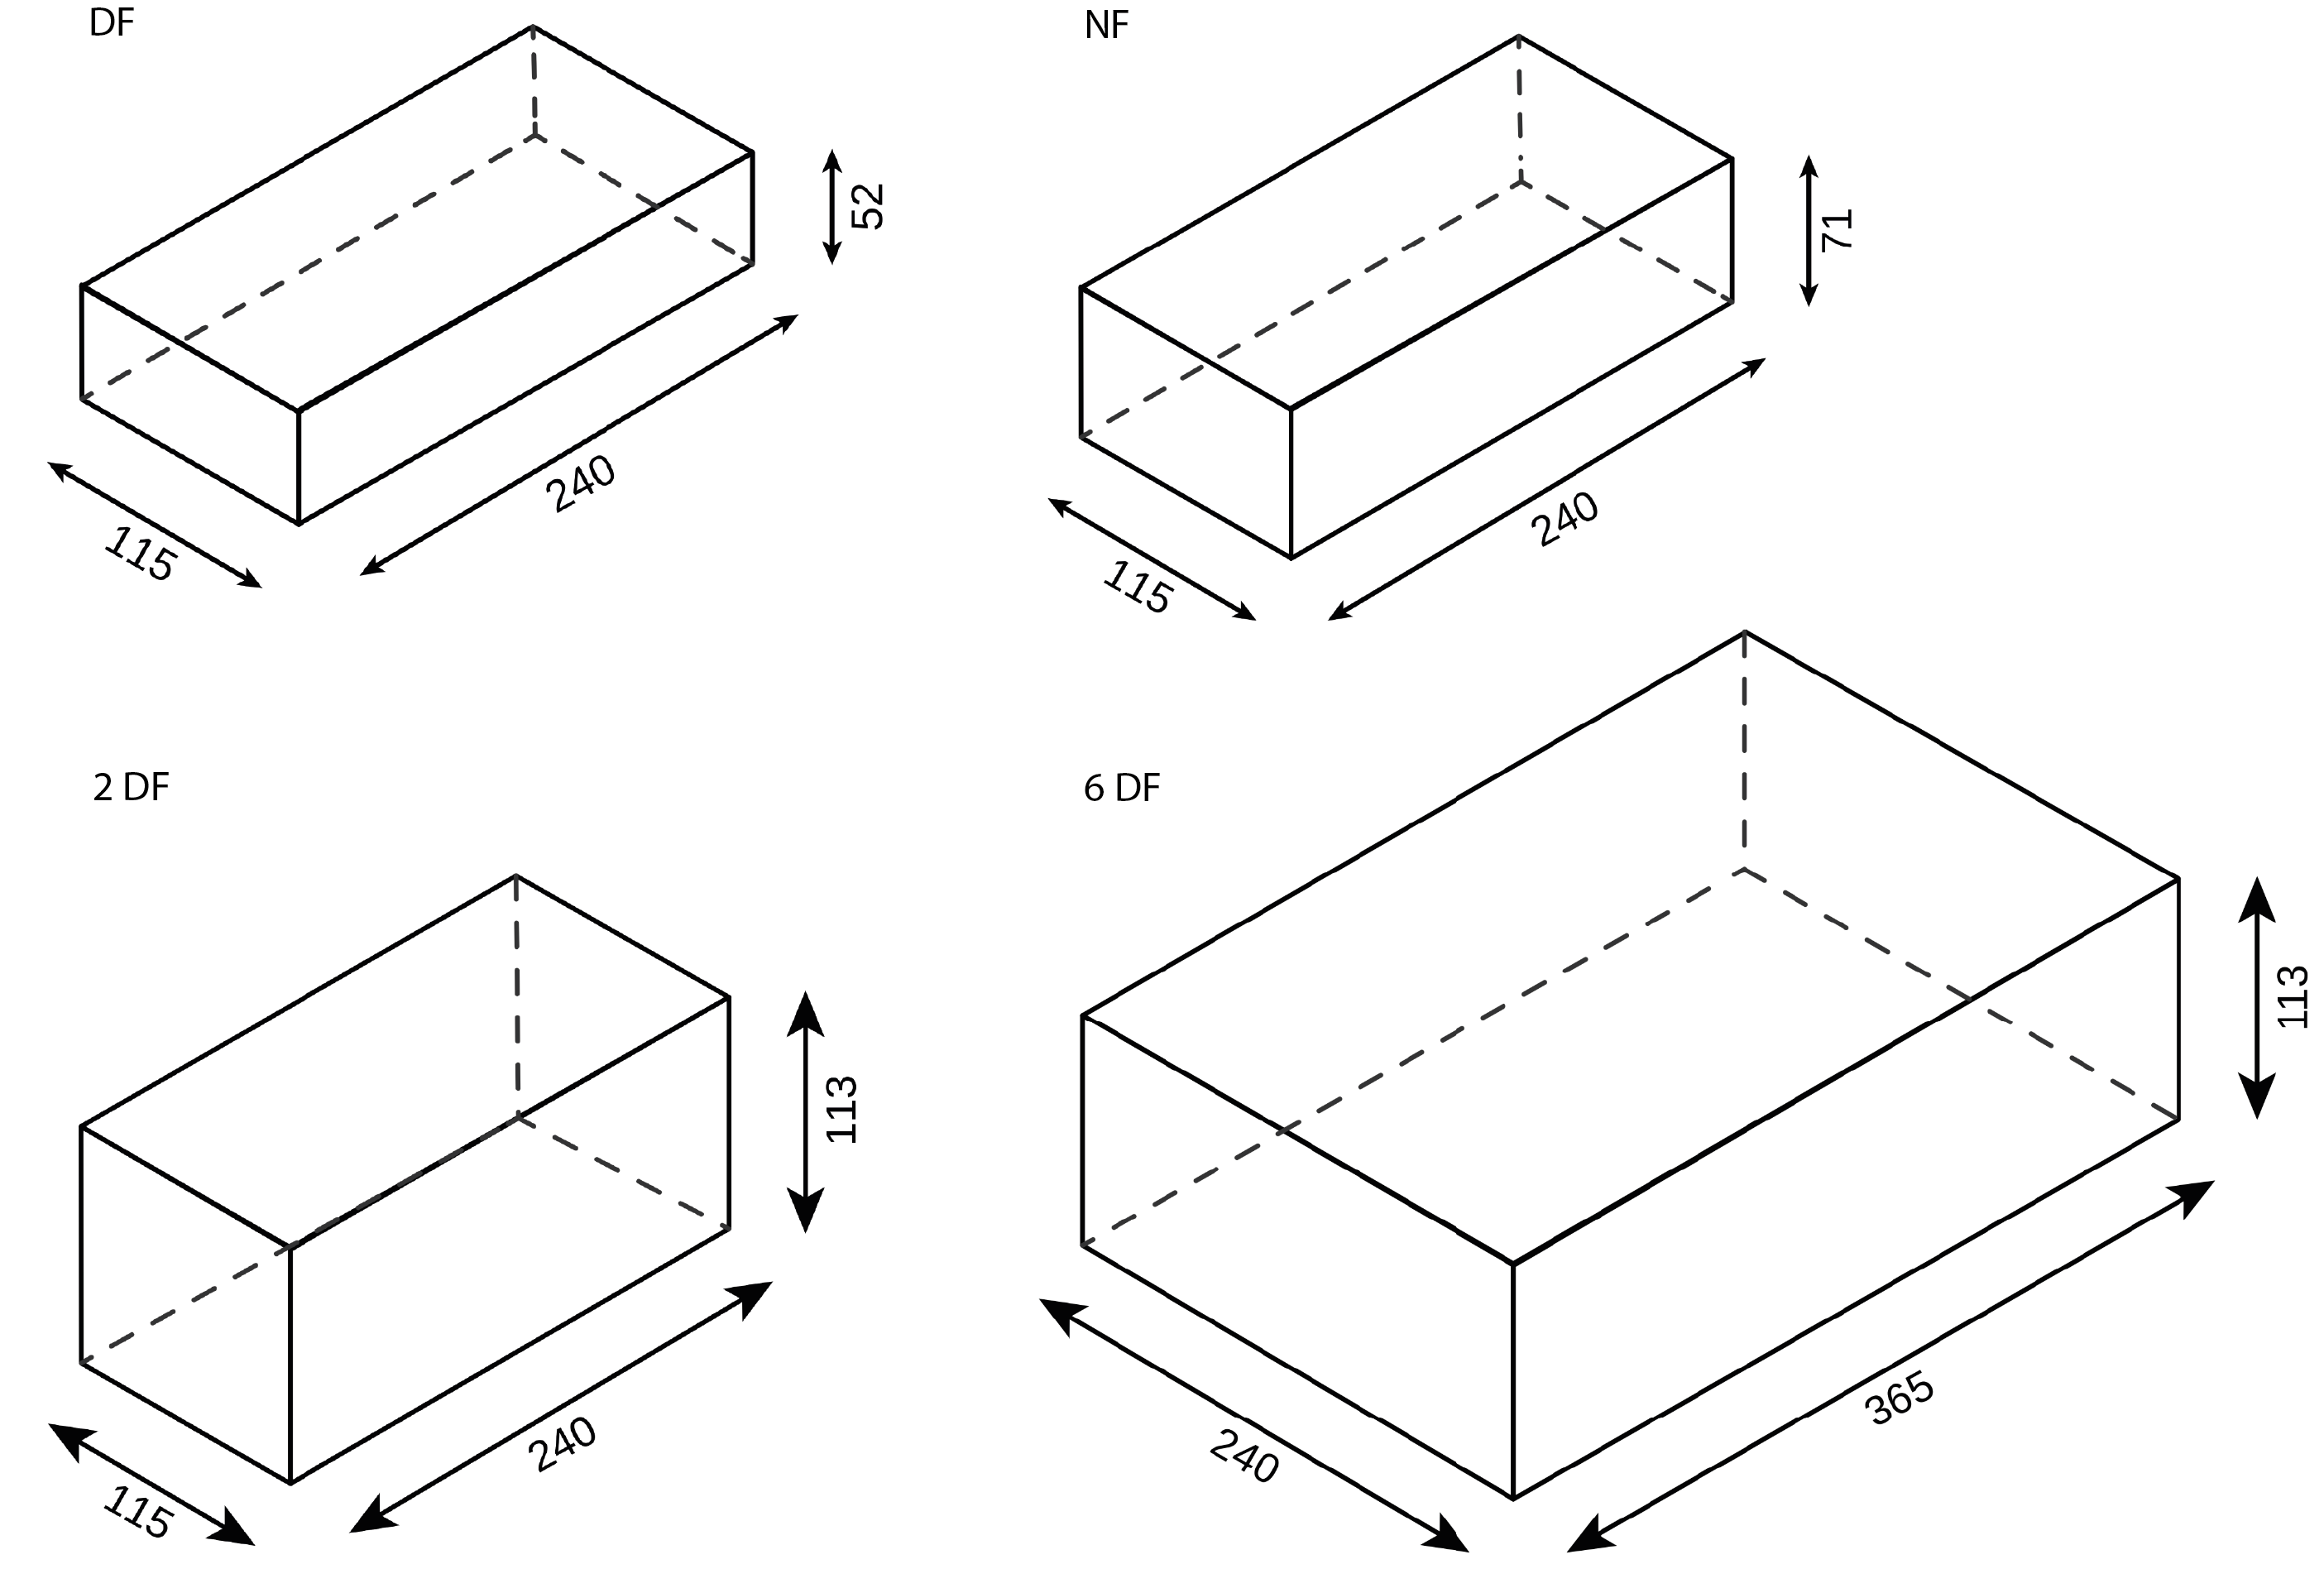
\includegraphics[width=0.8\columnwidth]{fig/Ziegelsteinformate DF NF 2DF 6DF.png}
    \caption{Darstellung verschiedener Steinformate nach DIN 4172 (Baunennmaß in Millimetern)~\cite{Steinfor38:online}}
    \label{fig:basics:Steinformate}
\end{figure}
\begin{figure}[ht]
  \centering
  \includegraphics[width=0.5\columnwidth]{fig/Oktametrische Maßordnung.png}
  \caption{Besondere Eigenschaften der oktametrischen Maßordnung~\cite{Moro2021}}
  \label{fig:basics:OktametrischeMassordnung}
\end{figure}
Daraus gehen insbesondere folgende zwei Formate für Ziegelsteine hervor:
Das Normalformat (NF) mit \(240\times115\times71 mm\) und das Dünnformat (DF) mit \(240\times115\times52 mm\) (Länge$\times$Breite$\times$Höhe)~\cite{Moro2021}.
Alle anderen Formate werden mithilfe dieser beiden Grundsteine angegeben.
So sind zum Beispiel die in Abbildung~\ref{fig:basics:Steinformate} gezeigten 2 DF und 6 DF Steine eine Kombination aus mehreren Steinen im Dünnformat.
Dabei sieht die Norm ein Fugenmaß von \(10 mm\) für Stoßfugen (vertikal) und \(12 mm\) for Lagerfugen (horizontal) vor.
Für Systeme, die eine schmalere oder keine Fuge benötigen, werden entsprechend größere Steine hergestellt, um der Maßordnung weiterhin zu entsprechen.
Durch Einhalten eines Systems ist man zusätzlich in der Lage Türen und Fenster an die daraus entstehenden Öffnungsgrößen anzupassen und vermeidet dadurch zeitaufwendiges, nachträgliches Anpassen.
Da Höhe, Breite und Länge der Steine zusammen mit den dazwischenliegenden Fugen aufgrund des Maßsystems jeweils Vielfache voneinander sind, ergeben sich viele Möglichkeiten zur Aufschichtung und Aneinanderreihung der Bausteine.
Einige davon sind in Abbildung~\ref{fig:basics:OktametrischeMassordnung} zu sehen und sind gleichzeitig Beispiele für einen sogenannten \textit{Mauerwerksverband}.

\subsection{Mauerwerksverband}
\label{basics:Mauerwerksverband}
Als Mauerwerksverband bezeichnet man bestimmte, gleichmäßige Anordnungen von Mauersteinen, um einen homogenen Mauerwerkskörper zu erreichen~\cite{Mauerwer39:online}.
Damit kann eine gleichmäßige Kraftverteilung innerhalb der Mauer gewährleistet werden.
Eine wichtige Rolle nimmt dabei das Überbindemaß ein, welches die Mindestüberlappung von Mauersteinen aus zwei Schichten der Mauer vorgibt.
Für das planmäßige Überbindemaß \(l_{ol}\) gilt für übliche Mauersteine mit Schichthöhen 
\(h_{u} \leq 249 mm\) 
nach DIN EN 1996-1-1: 
\(l_{ol} \geq 0,4h_{u} \geq 45 mm\)
~\cite{Bemessun72:online}\cite{DIN_EN_1996_1_1}.
Zudem wird darin die Mindestwanddicke für tragendes Mauerwerk, \glqq{}sofern aus Gründen der Standsicherheit, der Bauphysik oder des Brandschutzes nicht größere Dicken erforderlich sind\grqq{}~\cite{Bemessun72:online}, auf 
\(t_{min} = 115 mm\) 
festgelegt~\cite{DIN_EN_1996_1_1}.
Dies ist, wie in Abbildung~\ref{fig:basics:Steinformate} zu sehen, exakt die Breite der kleinsten Ziegelformate NF und DF.
Man unterscheidet zwei Arten von Mauerwerk: das Einsteinmauerwerk und das Verbandsmauerwerk.
Wie schon dem Namen zu entnehmen, handelt es sich beim Einsteinmauerwerk und ein Mauerwerk, bei welchem die Wanddicke der Steindicke entspricht.
Hier muss das Überbindemaß lediglich über die Wandlängsrichtung eingehalten werden.
Bei Verbandsmauerwerk gilt dies zusätzlich für die Wandquerrichtung~\cite{05maurer1:online}.
Einige Beispiele sind in Abbildung~\ref{fig:basics:verbaende} zu sehen.
\begin{figure}[htb]
  \begin{subfigure}[b]{0.5\columnwidth}
    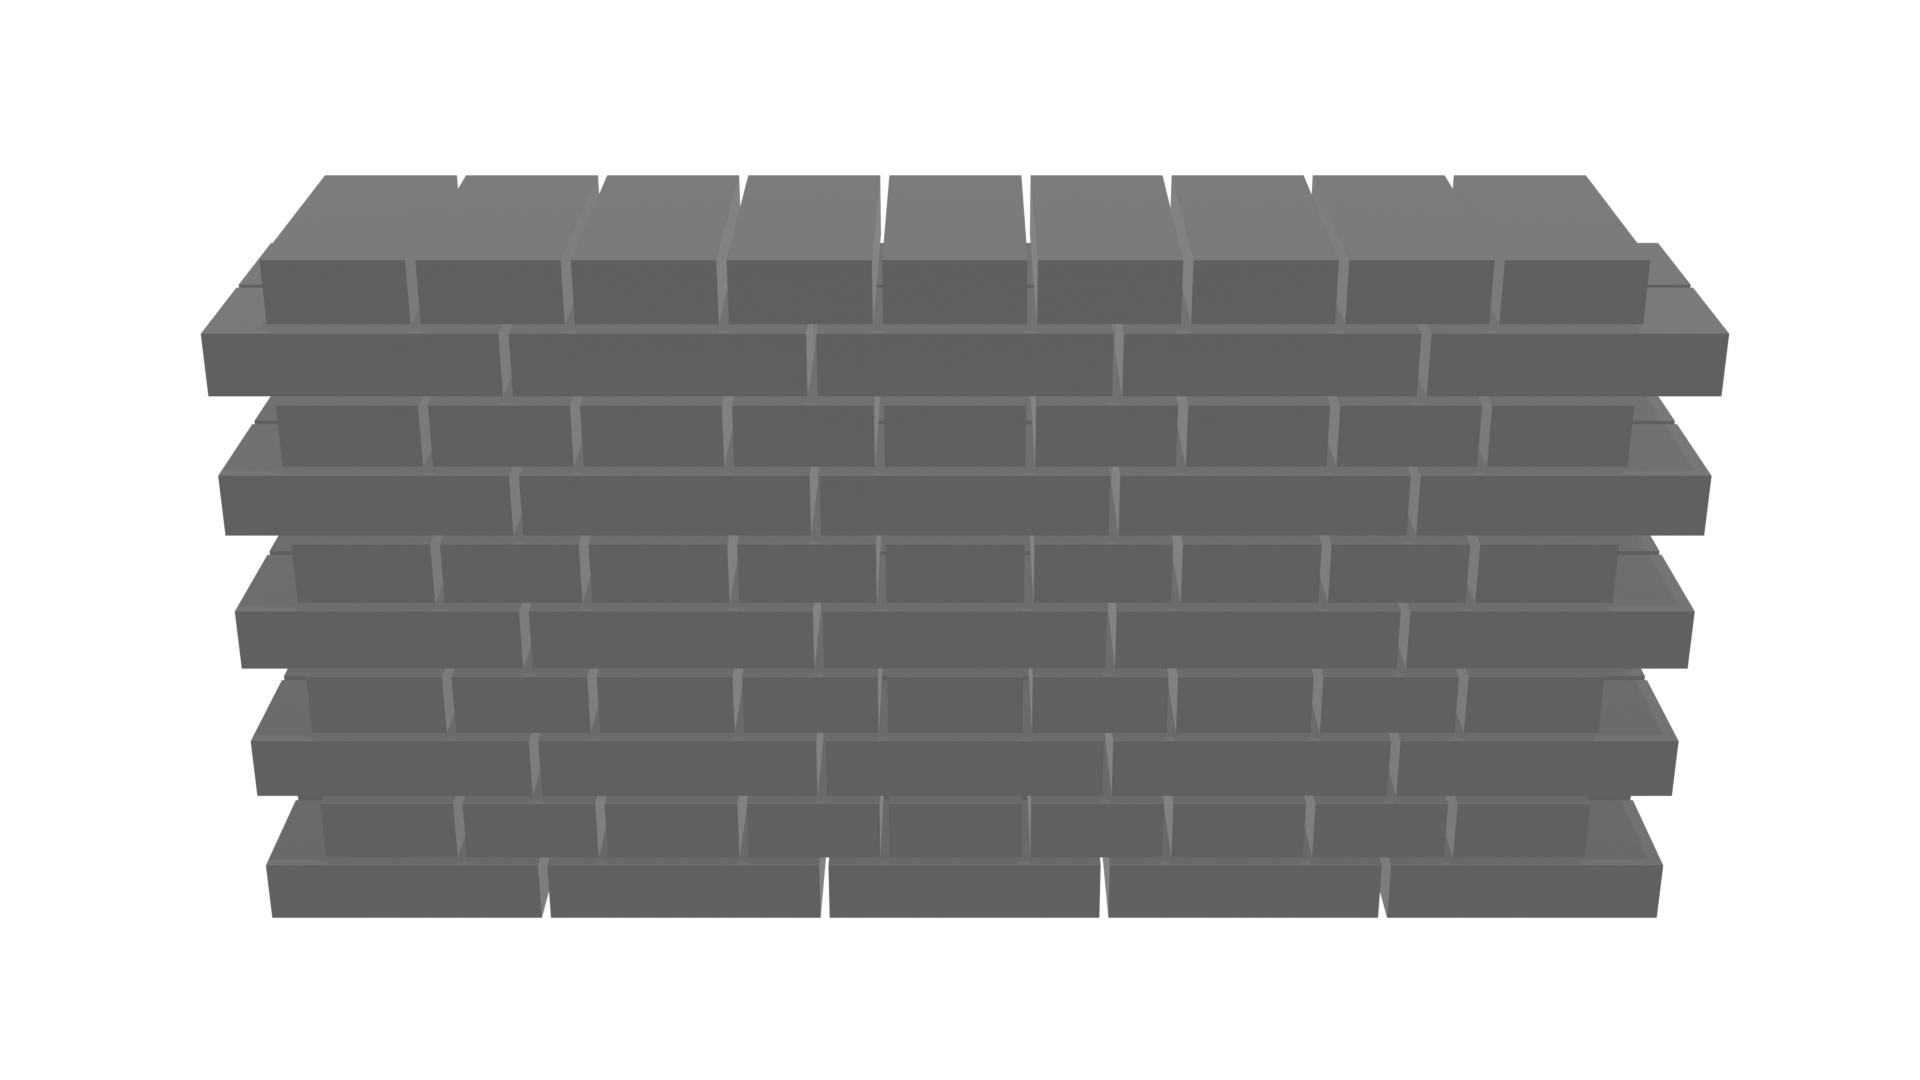
\includegraphics[width=\columnwidth]{fig/blockverband.png}
    \caption{Blockverband.}
    \label{fig:basics:blockverband}
  \end{subfigure}
  \hfill
  \begin{subfigure}[b]{0.5\columnwidth}
    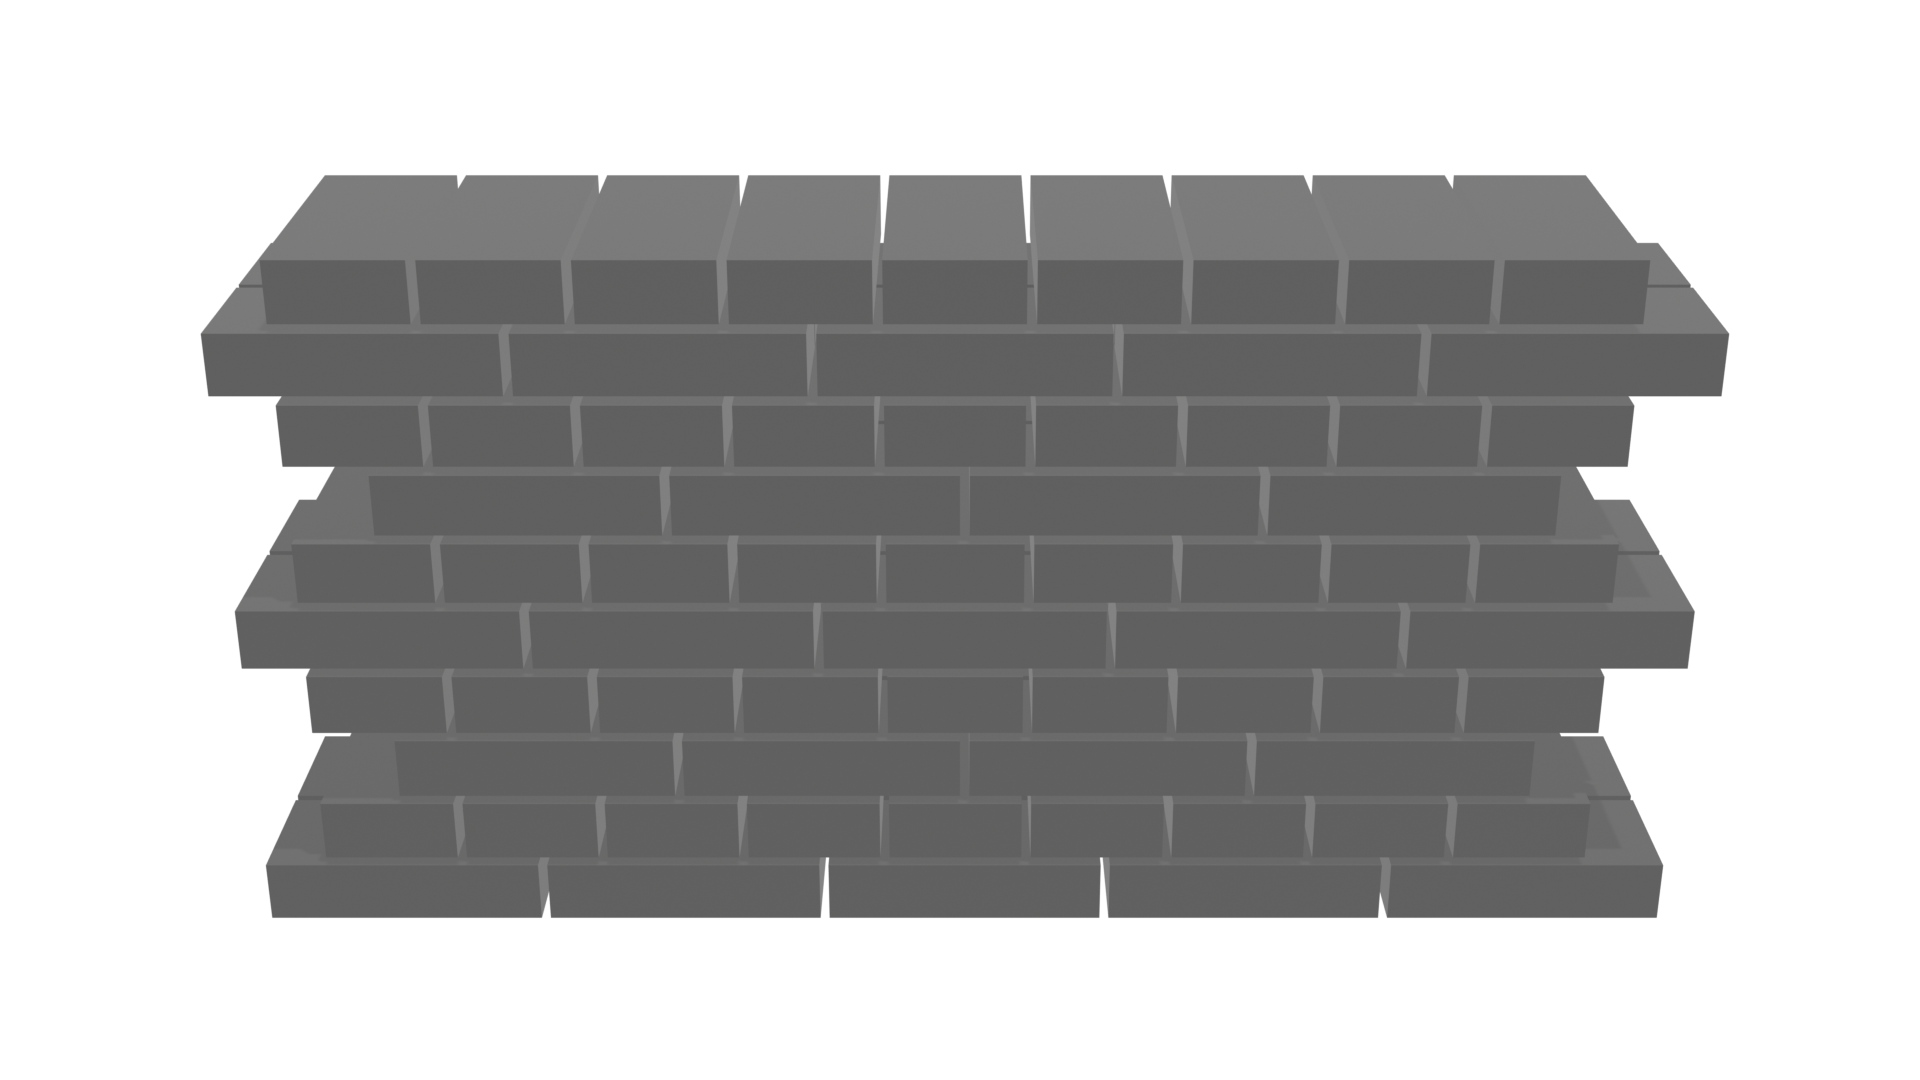
\includegraphics[width=\columnwidth]{fig/kreuzverband.png}
    \caption{Kreuzverband.}
    \label{fig:basics:kreuzverband}
  \end{subfigure}
  \begin{subfigure}[b]{0.5\columnwidth}
    \includegraphics[width=\columnwidth]{fig/läuferverband025_mittig.png}
    \caption{Mittlerer Läuferverband \textit{(1/4 Versatz).}}
    \label{fig:basics:laeuferverband_mittig}
  \end{subfigure}
  \begin{subfigure}[b]{0.5\columnwidth}
    \includegraphics[width=\columnwidth]{fig/läuferverband033_schleppend.png}
    \caption{Schleppender Läuferverband \textit{(1/3 Versatz).}}
    \label{fig:basics:laeuferverband_schleppend}
  \end{subfigure}
  \begin{subfigure}[b]{0.5\columnwidth}
    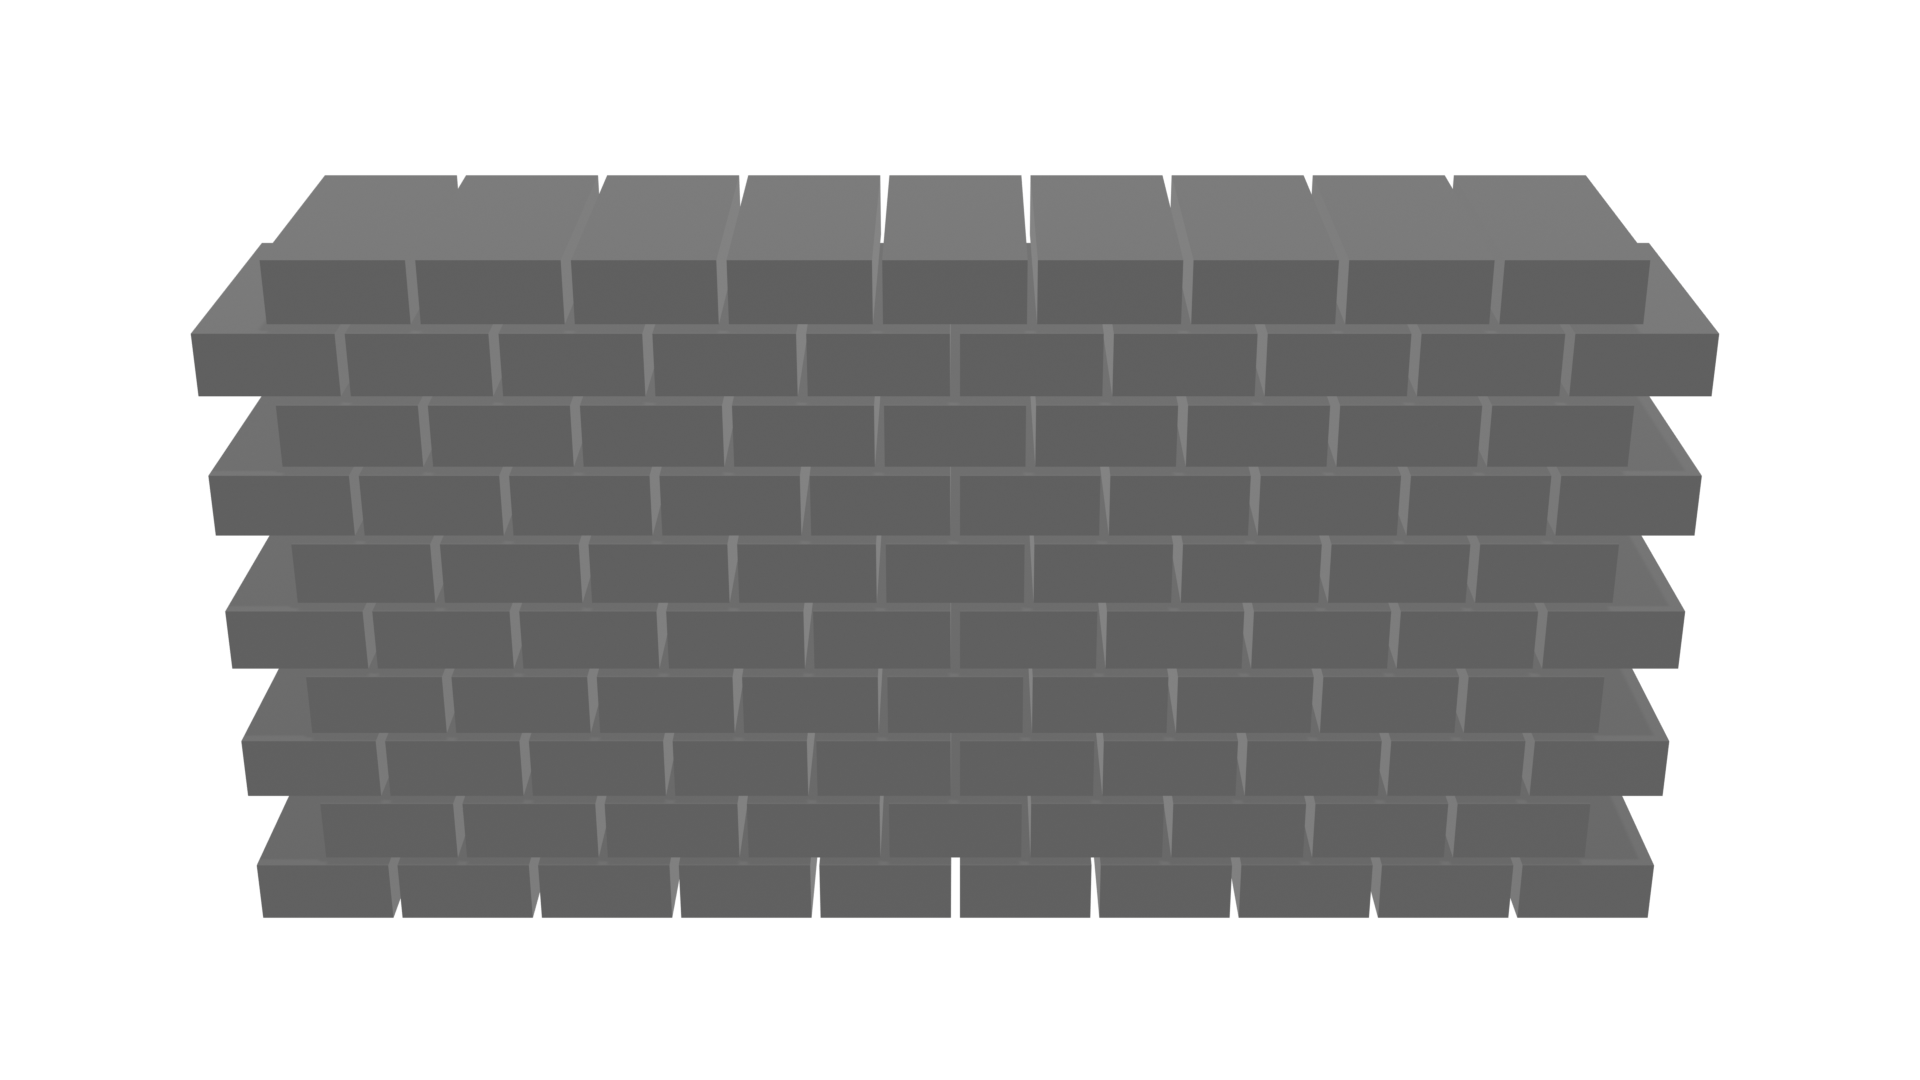
\includegraphics[width=\columnwidth]{fig/kopfverband.png}
    \caption{Kopf/Binderverband.}
    \label{fig:basics:binderverband}
  \end{subfigure}
  \begin{subfigure}[b]{0.5\columnwidth}
    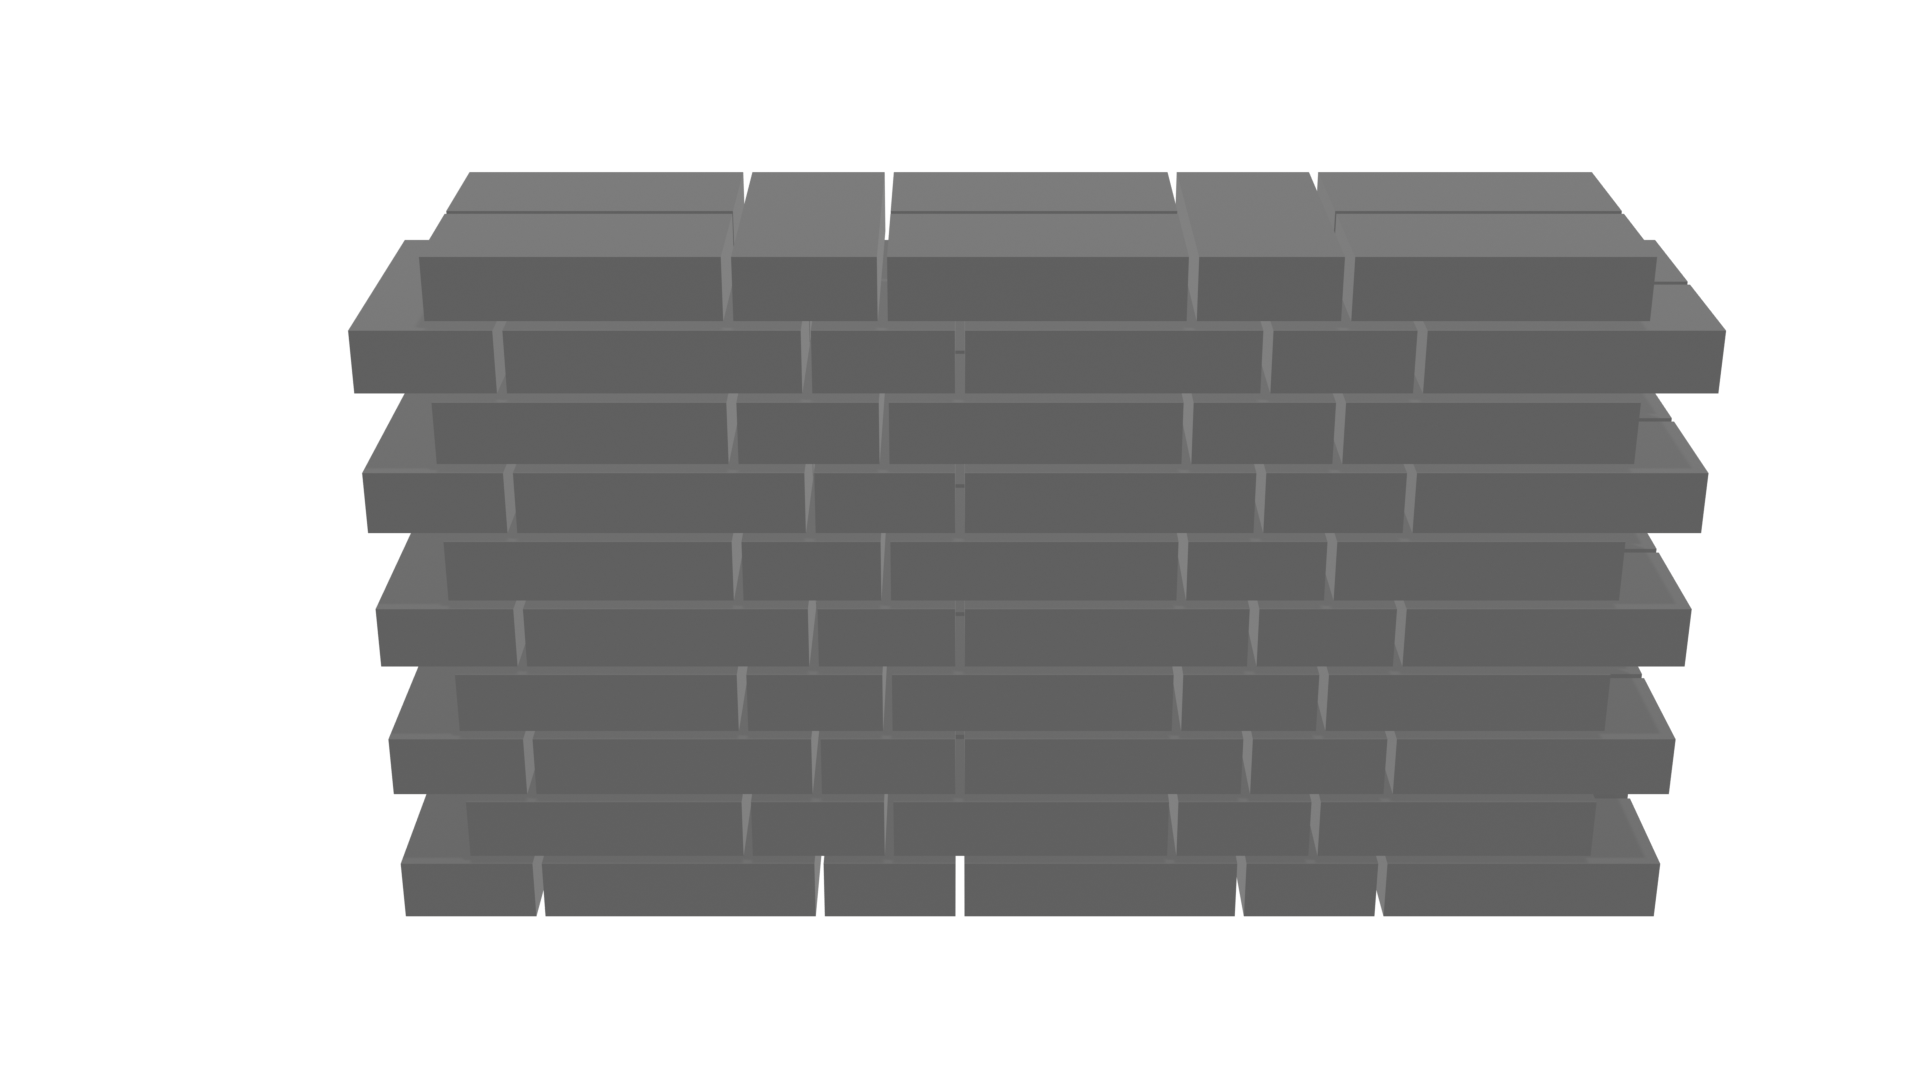
\includegraphics[width=\columnwidth]{fig/gotischerverband.png}
    \caption{Gotischer Verband.}
    \label{fig:basics:gotischer_verband}
  \end{subfigure}
  \caption{Typische Mauerwerksverbände.}
  \label{fig:basics:verbaende}
\end{figure}
Als Wandstück wird von nun an ein gerader Wandabschnitt bezeichnet.
Dieser hat eine Länge, eine Höhe und durch einen vorgegebenen Bausteintyp und einem gewünschten Verband eine gewisse Breite.
Treffen zwei oder mehrere Wandstücke aufeinander, so gilt es diese dem Überbindemaß entsprechend miteinander zu verzahnen.
Dabei treten verschiedene Sonderfälle auf, die für unterschiedliche Verbände nach unterschiedlichen Lösungen verlangen:

\begin{enumerate}
  \item \textbf{Ecken} werden durch zwei sich an Wandenden berührenden, meist rechtwinklig zueinanderstehenden Wandstücken gebildet.
  \item \textbf{Kreuzungen} stellen zum Beispiel zwei sich kreuzende Wandstücke dar.
  \item \textbf{T-Kreuzungen} entstehen, wenn ein Wandende des einen Wandstücks auf einer anderen Wand steht.
  Sowohl bei Kreuzungen als auch T-Kreuzungen kann auf das aufwendige Verahnen verzichtet und stattdessen die sogenannte Stumpfstoßtechnik angewandt werden.
  Dabei werden Stahlanker zwischen der Wand und den darauf treffenden \glqq{}stumpfen\grqq{} Wandenden verwendet, um die beiden Wände sicher miteinander zu verbinden.
  \item \textbf{Wandenden} sind die \glqq{}Enden\grqq{} eines Wandstücks, die kein anderes Wandstück berühren.
  Dafür muss der verwendete Mauerwerksverband zu einem geraden Abschluss gebracht werden.
  Oftmals lässt sich das Anpassen der Bausteine (etwa durch zerschneiden) nicht vermeiden.
  \item \textbf{Öffnungen} innerhalb eines Wandstücks können in der selben Art behandelt werden, da der vorherrschende Verband in den betroffenen Schichten gerade unterbrochen werden muss.
  Über Öffnungen für Fenster und Türen wird ein sogenannter Sturz gelegt, welcher ebenfalls in den der Wand zugrunde liegenden Mauerwerksverband eingebunden werden muss.  
\end{enumerate}

Die Lösungen für die oben geannten Situationen variieren je nach angestrebten Mauerwerksverband und der verwendeten Modulgröße stark.
Einige Beispiele sind in Abbildung~\ref{fig:basics:mauerwerk_eckloesung} und Abbildung~\ref{fig:basics:Kreuzungsloesung} zu sehen~\cite{Moro2021}\cite{MaurerfibelKreuzungen:online}.
Während etwa beim Läuferverband darauf verzichtet werden kann Bausteine für Eckbereiche und Kreuzungen zu zerschneiden, ist dies für andere Verbände teilweise unumgänglich. 

\begin{figure}[ht]
  \centering
  \includegraphics[width=0.5\columnwidth]{fig/Eck- und Kreuzungslösungen.png}
  \caption{Lösungen für Ecken und T-Kreuzungen unterschiedlicher Verbände~\cite{Moro2021}}
  \label{fig:basics:mauerwerk_eckloesung}
\end{figure}

\begin{figure}[ht]
  % https://www.ks-maurerfibel.de/maurerfibel/4-mauerwerksverbaende/4-7-mauern-von-stoessen-und-kreuzungen/ 
  \centering
  \includegraphics[width=0.5\columnwidth]{fig/KreuzungslösungBeispiel.png}
  \caption{Lösung einer Kreuzung am Beispiel einer \glqq{}Wand aus 2 DF im Kreuz- und Blockverband\grqq{}~\cite{MaurerfibelKreuzungen:online}}
  \label{fig:basics:Kreuzungsloesung}
\end{figure}

%https://baulexikon.beuth.de/MAUERWERKSVERBAND.HTM
%https://www.bauprofessor.de/mauerwerksverband/
%DIN 1053-1 (wurde durch DIN EN 1996-1-1 ersetzt)
%anstoßendes Wandstück: der bereich an dem zwei wandsegmente aneinanderstoßen z.b eine ecke
%https://www.baunetzwissen.de/mauerwerk/fachwissen/planungsgrundlagen/verbaende-und-verzahnung-162752
%Verzahnung: aus https://baulexikon.beuth.de/VERZAHNUNG.HTM : Verzahnung, im Mauerwerksbau übliche Technik, beim Herstellen einer Wand eine Verbindungsstelle für eine später zu errichtende und in die bereits bestehende einzubindende Wand den Verbandsregeln entsprechend vorzubereiten. Es gibt Lochverzah- nung, stehende und liegende Verzahnung. Nur die letztgenannte Verzahnungsart gilt nach DIN 1053-1 als ausreichende Verbindung zwischen tragenden und aussteifenden Mauerwerkswänden
%Überbindemaß ist wichtig um Mauerwerksverbände zu bewerten
%https://www.mauerwerksbau-lehre.de/vorlesungen/1-grundlagen-und-baustoffe-des-mauerwerksbaus/13-wandkonstruktionen/132-mauerwerksverband-und-ueberbindemass
%TODO Rund Wände, keine 90 Grad Ecken

\section{LEGO}
\label{basics:lego}
Ein 1$\times$1 LEGO Stein hat eine quadratische Grundfläche von \(7.8mm\)$\times$\(7.8mm\).
Dies entspricht demnach dem Baunennmaß des 1$\times$1 LEGO Steins.
Zwischen zwei nebeneinander platzierten Steinen ist ein Abstand von  \(0.2mm\).
Daraus ergibt sich ein Baurichtmaß beziehungsweise ein Rastermaß von \(8mm\)$\times$\(8mm\).
In Abbildung~\ref{fig:basics:Lego 2x4 Brick} werden zur Veranschaulichung die Maße des populären 2$\times$4 Steines aufgeschlüsselt.
Die für ein dreidimensionales Maß noch fehlende Größe ist die Höhe der Steine.
Diese beträgt \(9.6mm\).
Der Abstand zwischen zwei übereinander gestapelten Steinen hängt von dem Druck ab, der beim Zusammenstecken geleistet wurde.
Dennoch kann dieser vernachlässigt, sprich als Abstand von \(0.0mm\) gewertet werden.

\begin{figure}[ht]
    \centering
    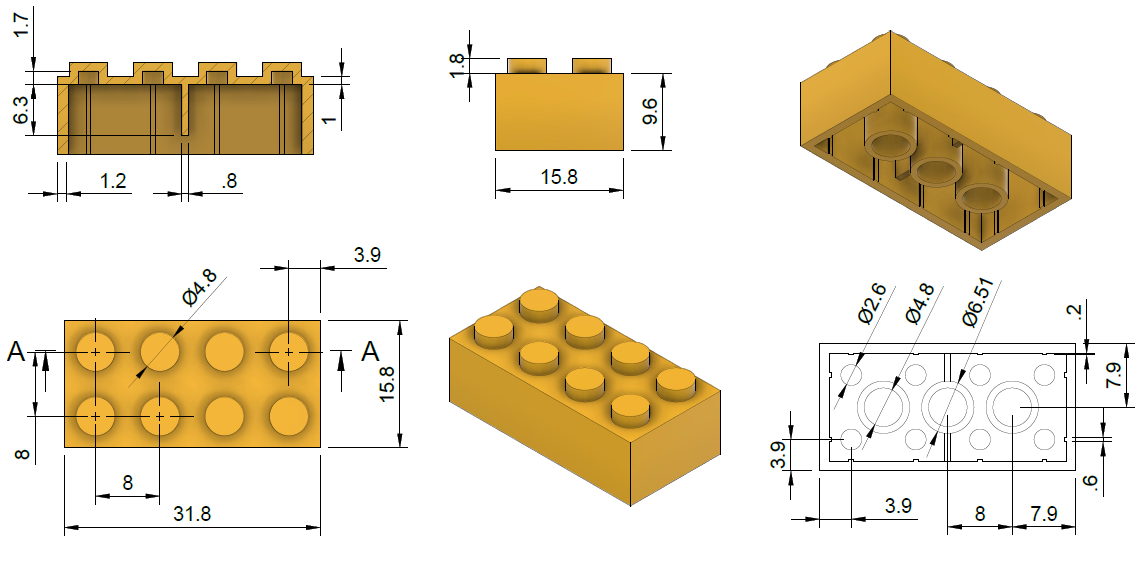
\includegraphics[width=0.8\columnwidth]{fig/LEGO 2x4 Brick horizontal.png}
    \caption{Maße des Standard 2$\times$4 LEGO Steins~\cite{LEGOBric2:online}}
    \label{fig:basics:Lego 2x4 Brick}
\end{figure}

\section{BRep}
\label{basics:brep}
Mal schauen

\section{Ontologien}
